\documentclass[final]{beamer}

% ====================
% Packages
% ====================

\usepackage[T1]{fontenc}
\usepackage{lmodern}
\usepackage[scale=1.2]{beamerposter}
\usetheme{gemini}
\usecolortheme{sjsu}
\usepackage{graphicx}
\usepackage{booktabs}
\usepackage{tikz}
\usetikzlibrary{arrows.meta, backgrounds, calc, fit, positioning}
\usepackage{pgfplots}
\pgfplotsset{compat=1.18}
\usepackage{anyfontsize}

% ====================
% Lengths
% ====================

% If you have N columns, choose \sepwidth and \colwidth such that
% (N+1)*\sepwidth + N*\colwidth = \paperwidth
\newlength{\sepwidth}
\newlength{\colwidth}
\setlength{\paperwidth}{48in} % A0 width: 46.8in
\setlength{\paperheight}{36in} % A0 height: 33.1in
\setlength{\sepwidth}{0.025\paperwidth}
\setlength{\colwidth}{0.3\paperwidth}

\newcommand{\separatorcolumn}{\begin{column}{\sepwidth}\end{column}}

% ====================
% Title
% ====================

\title{Probing acoustic information through transformer-based speech encoders}

\author{Vidhaat Dunna, Hahn Koo, Kelsey Kraus}

\institute[shortinst]{San José State University}

% ====================
% Footer (optional)
% ====================

\footercontent{
  \makebox[\dimexpr\paperwidth-2\sepwidth\relax][c]{%
    \href{https://sjsu.edu/}{https://sjsu.edu} \hfill
    {Department of Linguistics and Language Development}}}
% (can be left out to remove footer)

% ====================
% Logo (optional)
% ====================

% use this to include logos on the left and/or right side of the header:
\logoright{\includegraphics[height=3cm]{sjsu_logos/sjsu_cs.png}}
\logoleft{
\includegraphics[height=3cm]{sjsu_logos/DEPT_LINGLANG_Gold_Reversed.png}}
% \logoleft{
\includegraphics[height=5cm]{sjsu_logos/SJSU_University_monogram_Reversed.png}}
% \logoright{
\includegraphics[height=6cm]{sjsu_logos/SpartanSpirit[reversed].png}}

% diagram setup
\definecolor{encBlue}{RGB}{0,96,168}
\definecolor{encLightBlue}{RGB}{211,226,240}
\definecolor{encOrange}{RGB}{224,153,0}
\definecolor{encLightOrange}{RGB}{255,238,194}
\colorlet{encoderblue}{sjsublue!35}
\colorlet{borderblue}{sjsublue}
\colorlet{embedgray}{boxgray}
\colorlet{orangehi}{sjsugold!55}
\colorlet{goldlight}{sjsugold!45}
\colorlet{gold}{sjsugold}
\colorlet{probe}{sjsublue}

\tikzset{
  enc-arrow/.style={-{Latex[length=2.4mm]}, line width=0.7pt},
  enc-io/.style={
    draw=encBlue, fill=white, very thick, rounded corners=1pt,
    align=center, text width=79mm, minimum width=83mm,
    minimum height=34mm, inner sep=1mm,
    font=\fontsize{34}{39}\selectfont
  },
  enc-stage/.style={
    draw=encBlue, fill=encLightBlue, very thick, rounded corners=1pt,
    align=center, text width=79mm, minimum width=83mm,
    minimum height=34mm, inner sep=1mm,
    font=\fontsize{34}{39}\selectfont
  },
  enc-prep/.style={
    draw=encBlue, fill=encLightBlue, very thick, rounded corners=1pt,
    align=center, minimum width=31mm, minimum height=14mm,
    font=\small
  },
  enc-frame/.style={
    draw=encBlue, fill=encLightBlue, very thick, rounded corners=1pt,
    inner sep=3mm
  },
  enc-layer/.style={
    draw=black!45, fill=white, thick, rounded corners=0.5pt,
    align=center, minimum width=35mm, minimum height=7mm,
    font=\scriptsize
  },
  enc-orange/.style={
    draw=encOrange, fill=encLightOrange, very thick, rounded corners=1pt,
    align=center, text width=79mm, minimum width=83mm,
    minimum height=34mm, inner sep=1mm,
    font=\fontsize{34}{39}\selectfont
  },
  enc-context/.style={
    draw=black!55, fill=black!3, dashed, thick, rounded corners=1pt,
    align=center, text width=79mm, minimum width=83mm,
    minimum height=34mm, inner sep=1mm,
    font=\fontsize{34}{39}\selectfont
  },
  enc-context-frame/.style={
    draw=black!55, fill=none, dashed, thick, rounded corners=1pt,
    inner sep=5mm
  },
  enc-output/.style={
    draw=encBlue, fill=encBlue!10, very thick, rounded corners=1pt,
    align=center, minimum width=28mm, minimum height=13mm,
    font=\fontsize{8}{10}\selectfont
  },
  enc-label/.style={font=\bfseries\small, align=center},
  enc-note/.style={font=\scriptsize, align=center}
}

% ====================
% Body
% ====================

\begin{document}

\begin{frame}[t]
\begin{columns}[t]
\separatorcolumn

\begin{column}{\colwidth}

  \begin{block}{Abstract}

    Although audio encoders are used in many speech applications, it is unclear how they use linguistic features
    in their input to perform language understanding tasks. 
    Classifiers (probes) can be used to predict high-level information from encoders’ internal layers, but probing 
    methods are not standardized, making results difficult to compare. In this experiment, we investigate if probe
    performance depends on encoder pretraining.

  \end{block}

  \begin{block}{Background}

    Audio encoders are used to generate vectors that encode the information present in one "frame", around 20ms of 
    audio. We choose to probe three encoders that differ in their training strategies:

    \begin{alertblock}{Wav2Vec2.0 (12 layers, 768 dimensions)}
      Wav2vec2 first has unsupervised pretraining on untranscribed audio, then is fine-tuned on transcribed speech.
      This encoder is intended to be fine-tuned for specific applications.
      \par\noindent\makebox[\linewidth][c]{\resizebox{\linewidth}{!}{%
      \begin{tikzpicture}[node distance=5mm and 5mm]
  \node[enc-io] (wvin) {audio};
  \node[enc-stage, right=of wvin] (wvenc)
    {convolutional\\network};
  \node[enc-stage, right=of wvenc] (wvcontext)
    {Transformer\\blocks};
  \node[enc-context, right=of wvcontext] (wvdec)
    {generic\\decoder};

  \draw[enc-arrow] (wvin) -- (wvenc);
  \draw[enc-arrow] (wvenc) -- (wvcontext);
  \draw[enc-arrow] (wvcontext) -- (wvdec);
\end{tikzpicture}
      }}\par
    \end{alertblock}
    \begin{alertblock}{Whisper-small/large-v3 (12/32 layers, 768/1280 dimensions)}
      The Whisper encoders undergo supervised multitask pretraining on transcribed audio along with a dedicated
      decoder. 
      % Tasks that the encoder-decoders are trained for include transcription, translation into English, 
      % speech detection, and language identification. 80-channel log-magnitude mel-spectrogram 25ms windows with
      % stride of 10ms.
      \par\noindent\makebox[\linewidth][c]{\resizebox{\linewidth}{!}{%
      \begin{tikzpicture}[node distance=5mm and 5mm]
  \node[enc-io] (whin) {log-mel\\spectrogram};
  \node[enc-stage, right=of whin] (whconv)
    {convolutional\\network};
  \node[enc-stage, right=of whconv] (whenc)
    {Transformer\\blocks};
  \node[enc-context, right=of whenc] (whdec)
    {multitask\\decoder};

  \draw[enc-arrow] (whin) -- (whconv);
  \draw[enc-arrow] (whconv) -- (whenc);
  \draw[enc-arrow] (whenc) -- (whdec);
\end{tikzpicture}
      }}\par
    \end{alertblock}
    \begin{alertblock}{Voxtral (32 layers, 1280 dimensions)}
      Voxtral shares an architecture with Whisper-large-v3, but is fine-tuned along with an encoder adapter in order
      to be used as input for an LLM.
      \par\noindent\makebox[\linewidth][c]{\resizebox{\linewidth}{!}{%
      \begin{tikzpicture}[node distance=5mm and 5mm]
  \node[enc-io] (vxin) {log-mel\\spectrogram};
  \node[enc-stage, right=of vxin] (vxenc)
    {whisper L-v3\\encoder};
  \node[enc-orange, right=of vxenc] (vxadapt)
    {audio\\adapter};
  \node[enc-context, right=of vxadapt] (vxllm)
    {multimodal\\LLM};

  \draw[enc-arrow] (vxin) -- (vxenc);
  \draw[enc-arrow] (vxenc) -- (vxadapt);
  \draw[enc-arrow] (vxadapt) -- (vxllm);
\end{tikzpicture}
      }}\par
    \end{alertblock}

  \end{block}

\end{column}

\separatorcolumn

\begin{column}{\colwidth}

  
  \begin{block}{Preprocessing}
    Clips from the TIMIT dataset are split at the segment-level, then passed through encoders. 
    Segment embeddings are averaged over the time dimension before being used to train fully-connected linear
    classifiers to predict manner of articulation and phone labels.

    % \begin{alertblock}{Time-averaged Frame Representations}
\begin{center}
\resizebox{\linewidth}{!}{%
\begin{tikzpicture}[x=1cm,y=1cm]

  % ---------------------------------------------------------------
  % Audio waveform
  % ---------------------------------------------------------------
  \node[font=\sffamily\fontsize{8}{10}\selectfont,align=center,text width=12.3cm] at (6.50,16.75)
    {\textcolor{blue!65!black}{audio:}\\ ``ambidextrous pickpockets accomplish more''};
  \node[anchor=north] at (6.50,16.48)
    {\includegraphics[width=12.3cm]{figures/speechRender.png}};

  % ---------------------------------------------------------------
  % Audio preprocessing and encoder flow
  % ---------------------------------------------------------------
  \draw[fill=encoderblue,draw=borderblue,line width=1.1pt]
    (0.45,10.75) rectangle (6.00,11.75);
  \node[font=\sffamily\fontsize{8}{10}\selectfont]
    at (3.225,11.25) {encoder preprocessor};

  \draw[very thick,-{Stealth[length=3mm]}]
    (3.225,12.15) -- (3.225,11.78);
  \draw[very thick,-{Stealth[length=3mm]}]
    (3.225,10.72) -- (3.225,10.05);

  % ---------------------------------------------------------------
  % Encoder stack
  % ---------------------------------------------------------------
\begin{scope}[yshift=-6mm]
  \draw[fill=encoderblue,draw=borderblue,line width=1.1pt]
    (0.10,1.72) rectangle (6.12,10.62);
  \node[font=\sffamily\fontsize{14}{16}\selectfont] at (3.11,10.12) {encoder};
  \node[font=\fontsize{7}{8}\selectfont,align=center,text width=5.7cm] at (3.11,9.78)
    {(wav2vec/whisper-small/whisper-large/voxtral)};

  \fill[white] (0.27,8.00) rectangle (5.95,9.46);
  \node[font=\rmfamily\fontsize{10}{12}\selectfont] at (3.11,8.72) {transformer layer 1};

  \fill[embedgray] (0.30,6.65) rectangle (5.92,7.71);
  \fill[orangehi] (3.25,6.65) rectangle (3.53,7.71);
  \fill[orangehi] (4.50,6.65) rectangle (4.65,7.71);
  \node[font=\sffamily\fontsize{7}{8}\selectfont] at (3.11,7.18) {(time $\times$ encoder dimension)};

  \fill[white] (0.27,5.42) rectangle (5.95,6.84);
  \node[font=\rmfamily\fontsize{10}{12}\selectfont] at (3.11,6.13) {transformer layer 2};

  \fill[embedgray] (0.30,4.20) rectangle (5.92,5.22);
  \fill[orangehi] (3.25,4.20) rectangle (3.53,5.22);
  \fill[orangehi] (4.50,4.20) rectangle (4.65,5.22);
  \node[font=\sffamily\fontsize{7}{8}\selectfont] at (3.11,4.71) {(time $\times$ encoder dimension)};

  \node[font=\sffamily\fontsize{7}{8}\selectfont] at (3.11,4.04) {$\vdots$};

  \fill[white] (0.27,2.85) rectangle (5.95,3.88);
  \node[font=\rmfamily\fontsize{10}{12}\selectfont] at (3.11,3.36) {transformer final layer};

  \fill[embedgray] (0.30,1.88) rectangle (5.92,2.65);
  \fill[orangehi] (3.28,1.88) rectangle (3.57,2.65);
  \fill[orangehi] (4.53,1.88) rectangle (4.68,2.65);
  \node[font=\sffamily\fontsize{7}{8}\selectfont] at (3.11,2.26) {(time $\times$ encoder dimension)};

  % ---------------------------------------------------------------
  % Time-averaging embeddings
  % ---------------------------------------------------------------
  \draw[fill=goldlight,draw=gold,line width=1.1pt]
    (6.20,1.65) rectangle (8.35,10.58);
  \node[font=\sffamily\fontsize{7}{8}\selectfont,align=center,text width=2.0cm] at (7.275,10.15)
    {time-averaged\\embeddings};
  \node[font=\sffamily\fontsize{6}{7}\selectfont,align=center,text width=2.0cm] at (7.275,8.90)
    {(1 $\times$\\encoder\\dimension)};
  \foreach \yy in {7.40,5.15,2.05} {
    \fill[gold] (7.16,\yy) rectangle (7.47,\yy+.88);
  }

  % Arrows explicitly showing temporal averaging of internal states.
  \draw[very thick,-{Stealth[length=3mm]}]
    (5.95,7.18) .. controls (6.35,7.18) and (6.62,7.84)
    .. (7.16,7.84);
  \draw[very thick,-{Stealth[length=3mm]}]
    (5.95,4.71) .. controls (6.35,4.71) and (6.62,5.59)
    .. (7.16,5.59);
  \draw[very thick,-{Stealth[length=3mm]}]
    (5.95,2.26) .. controls (6.35,2.26) and (6.62,2.49)
    .. (7.16,2.49);

  % ---------------------------------------------------------------
  % Probe heads and output boxes
  % ---------------------------------------------------------------
  \foreach \yy/\label/\output in {8.05/MOA probe/moa labels,7.00/phone probe/phone labels,
                                  5.25/MOA probe/moa labels,4.20/phone probe/phone labels,
                                  2.82/MOA probe/moa labels,1.77/phone probe/phone labels} {
    \fill[probe] (8.78,\yy) rectangle (11.78,\yy+.94);
    \node[font=\sffamily\fontsize{8}{10}\selectfont,text=white,anchor=west]
      at (8.98,\yy+.47) {\label};
    \draw[line width=.8pt] (11.98,\yy) rectangle (13.55,\yy+.94);
    \node[font=\sffamily\fontsize{7}{8}\selectfont,align=center,text width=1.45cm]
      at (12.765,\yy+.47) {\output};
    \draw[thick,-{Stealth[length=2.6mm]}]
      (11.78,\yy+.47) -- (11.98,\yy+.47);
  }

  % Each frame-averaged embedding feeds its corresponding probe pair.
  \foreach \yy/\ya/\yb in {
    7.84/8.52/7.47,
    5.59/5.72/4.67,
    2.49/3.29/2.24
  } {
    \draw[thick,-{Stealth[length=2.6mm]}]
      (7.47,\yy) .. controls (7.95,\yy) and (8.15,\ya)
      .. (8.78,\ya);
    \draw[thick,-{Stealth[length=2.6mm]}]
      (7.47,\yy) .. controls (7.95,\yy) and (8.15,\yb)
      .. (8.78,\yb);
  }

  % Dashed grouping around the probe heads.
  \draw[dashed,line width=.9pt]
    (8.58,1.58) rectangle (13.68,9.25);
\end{scope}

\end{tikzpicture}
}
\end{center}    % \end{alertblock}
    % \begin{alertblock}{Probing}
    %   We train linear classifiers to predict manner of articulation and phone label from segment-averaged representations.
      
    % \end{alertblock}

  \end{block}
  % \begin{block}{A table of results, maybe?}

  %   \begin{table}
  %     \centering
  %     \begin{tabular}{l r r c}
  %       \toprule
  %       \textbf{Encoder} & \textbf{layer 0} & \textbf{final layer}\\
  %       \midrule
  %       Wav2Vec & 13.37 & 384,394 \\
  %       Whisper & 2.17 & 1,392 \\
  %       Voxtral & 3.14 & 83,742 \\
  %       \bottomrule
  %     \end{tabular}
  %     \caption{A table caption.}
  %   \end{table}

  % \end{block}

\end{column}

\separatorcolumn

\begin{column}{\colwidth}
  \begin{block}{Results}

    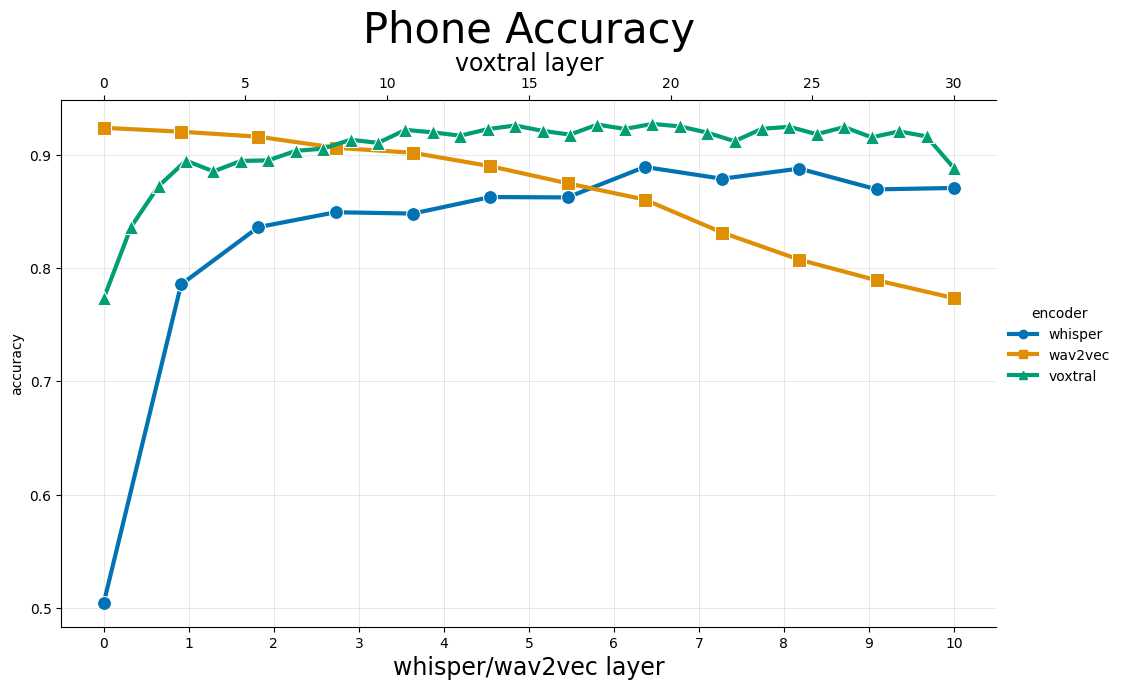
\includegraphics[width=\linewidth]{figures/layerwisePhoneAccuracy.png}\\
    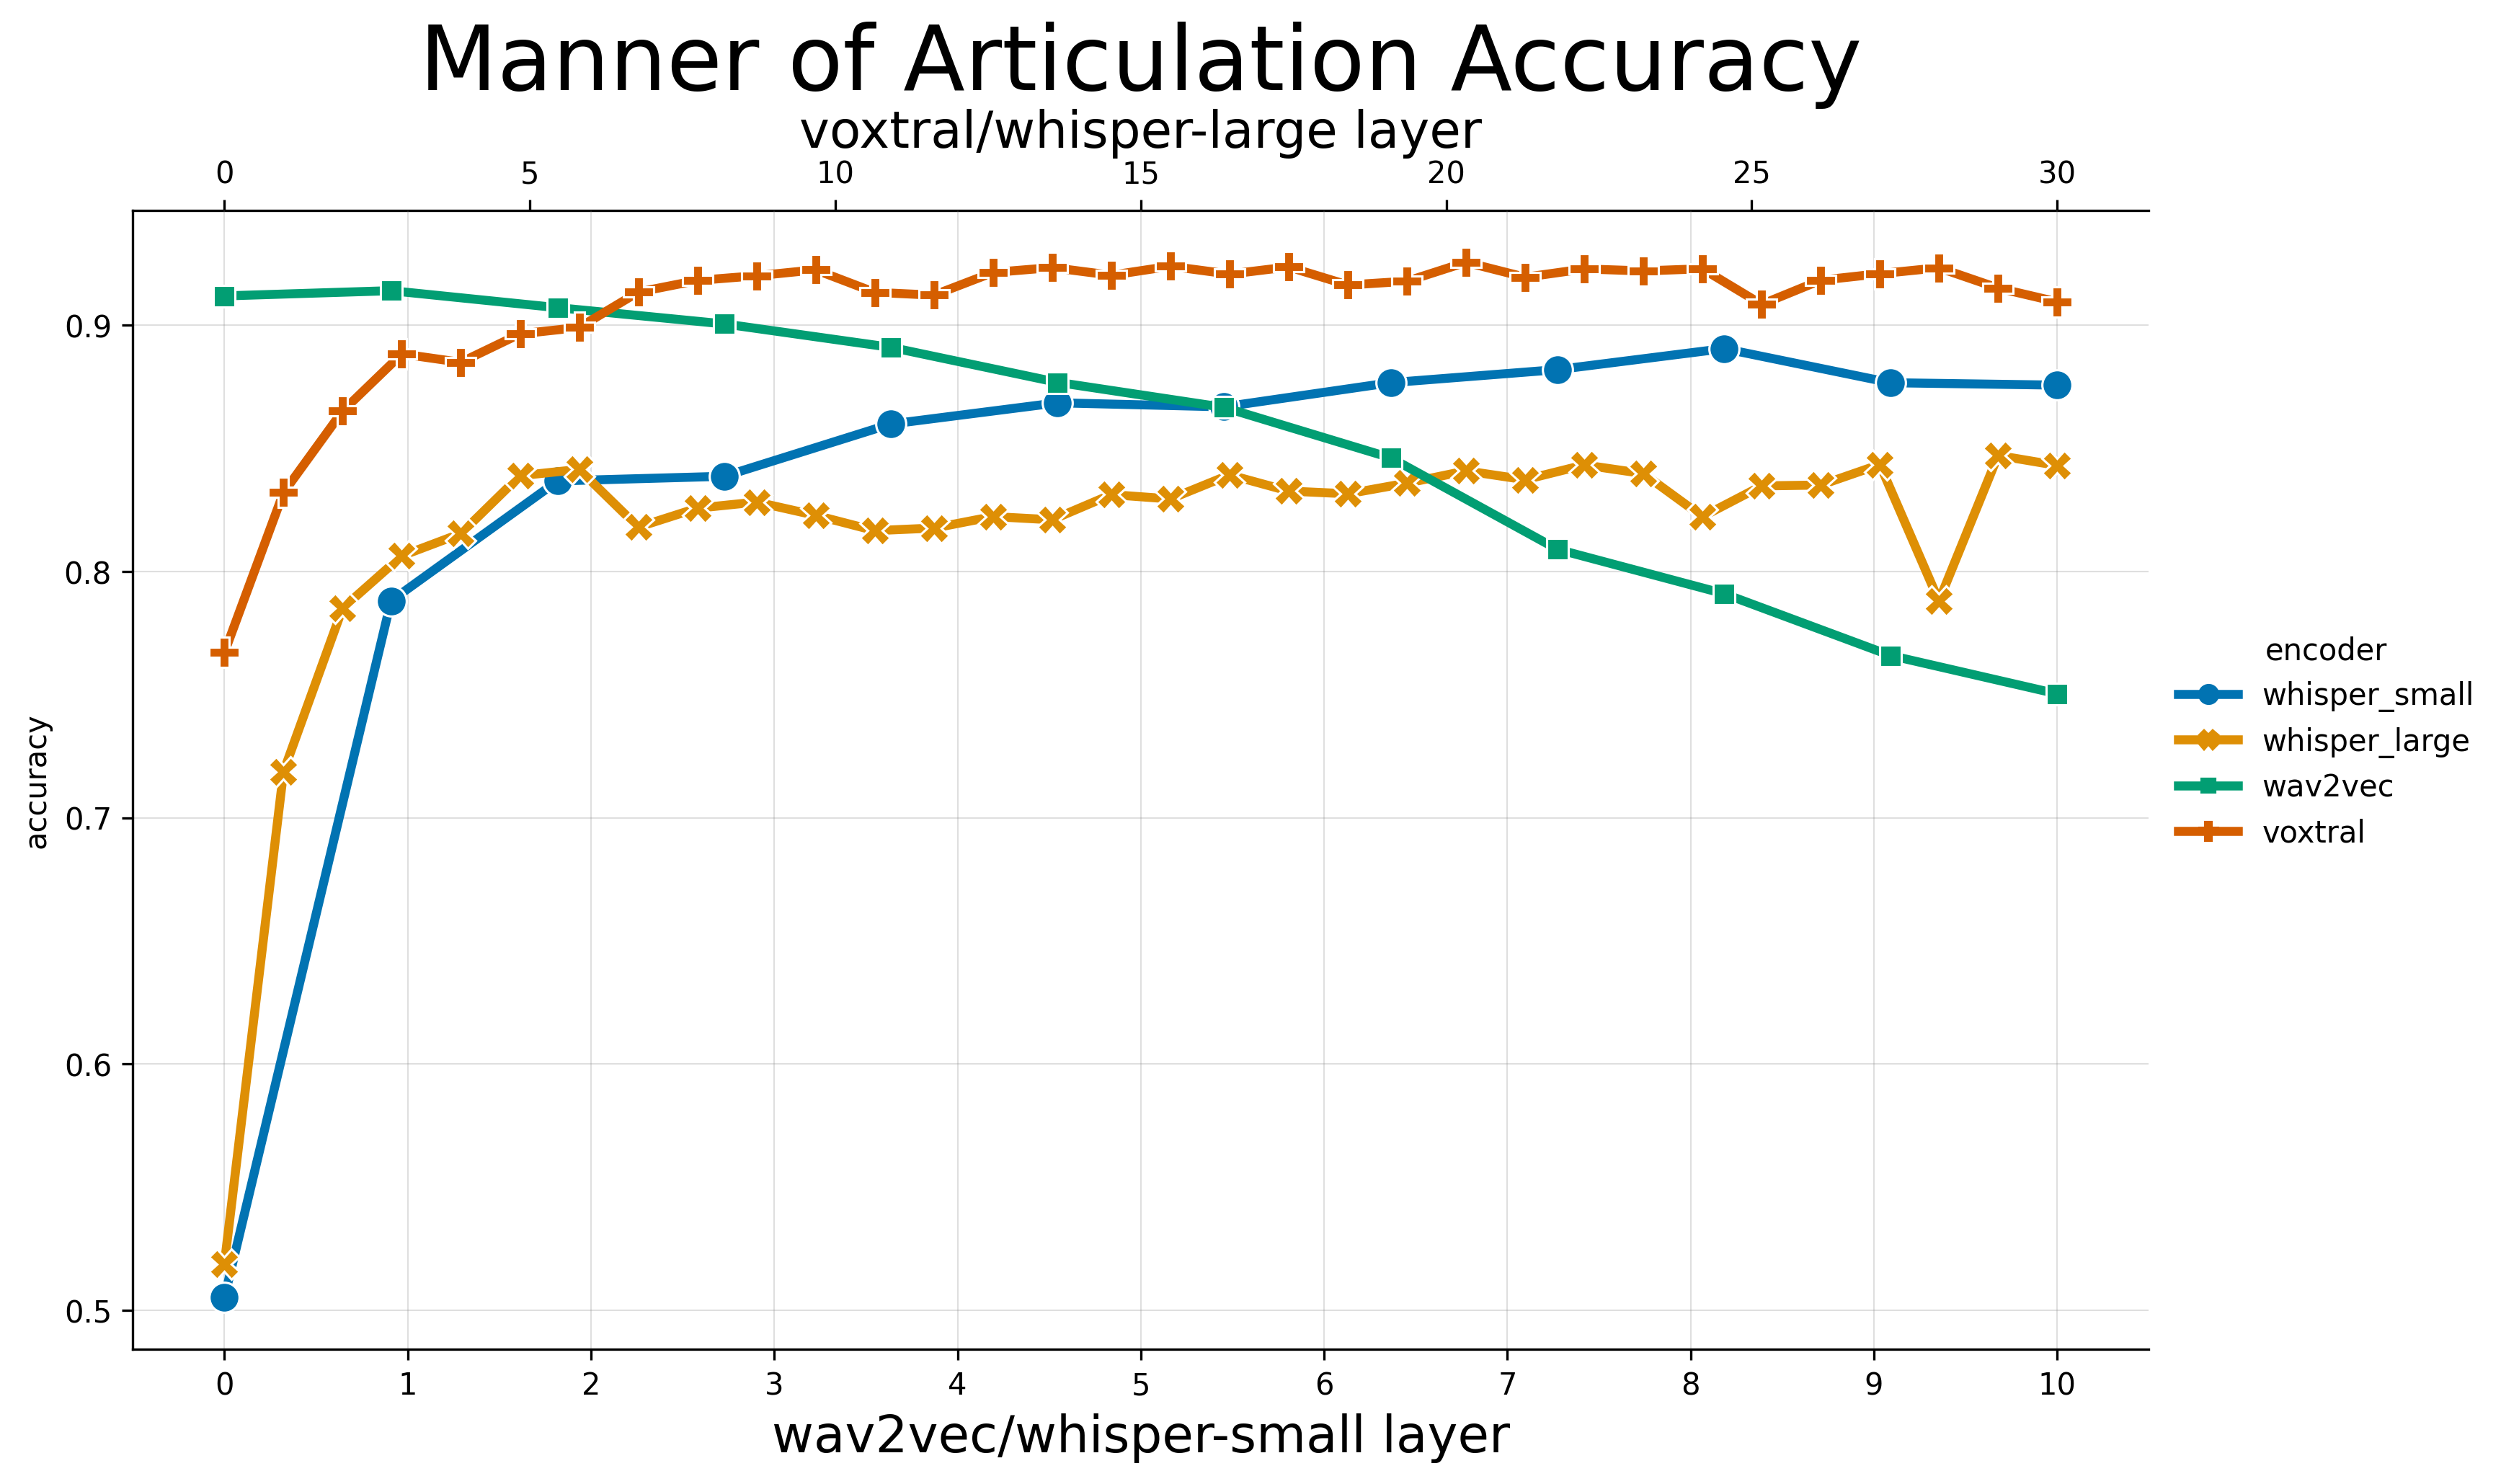
\includegraphics[width=\linewidth]{figures/layerwiseMoaAccuracy.png}\\

    Our wav2vec2 results challenge prior probing findings, suggesting that probing performance
    is sensitive to encoder training strategies and probe hyperparameters.

  \end{block}

  \begin{block}{References}
    {
      \tiny
      \nocite{*}
      \bibliographystyle{ieeetr}
      \vspace{-1ex}
      \bibliography{poster}
    }
  \end{block}
\end{column}

\separatorcolumn
\end{columns}
\end{frame}

\end{document}